\documentclass{report}
\usepackage[utf8]{inputenc}
\usepackage[top=2.5cm, left=2.3cm, right=2.7cm, bottom=3.0cm]{geometry}
\usepackage{accents}
%\usepackage{amsmath}
\usepackage{float}
\usepackage{hyperref}
\usepackage{pdfpages}
\usepackage{sectsty}
\usepackage{titlesec}
\usepackage{listings}
\usepackage{graphicx}
\graphicspath{ {./images/} }

\titleformat{\chapter}{\normalfont\huge}{\thechapter.}{20pt}{\huge\it}
\newcommand{\ubar}[1]{\underaccent{\bar}{#1}}
\newcommand{\e}[1]{\cdot10^{#1}}


\title{\huge Report FINAL \\ \Huge System Programming}
\author{\huge Baran Hasan Bozduman\\ \huge 171044036}
\date{\today}
\begin{document}
\maketitle
{\huge \textbf{Problem Definition} \\}

{\large  The required in this project a setting up client-server communication also some functionalities of SQL database (like SELECT, SELECT DISTINCT, UPDATE). The tricky part is there will be a thread pool  in the server so main thread will distribute the the queries to threads and each thread should be busy with the related client so there will be kind of producer consumer problem to manage available threads. Also since there will be other threads and we will use same database to read and write we should protect that and we can obtain that by using reader writer paradigm.\\}

{\huge \textbf{Design Decision} \\ \large .\\\large  \textbf{SERVER}\\
    Firstly I declare structs for queue and data set( its a struct and it has char* and size of char pointer of it) also i declare my threads as  global in an array and they are also struct but they just only keep thread ids\\ Inside of main I initialized a named semaphore to prevent double instantiating since they are initialized by kernel and are managed by them so it does not let to run it second time it returns an error instead of that so until you send SIGINT signal you can not run that program second time\\ Then u get terminal values by using get opt and check them in case of user can make mistake\\I read data and place in the memory and all the things are dynamic.\\I create a socket and bind an address on it. I initialized listen value as 100 so is there will be more connection than that it can not accept.\\I allocate space for threads according to pool size  and create threads, i send their ids as parameter so each thread will know which is which.\\ I determined the available thread numbers as pool size at first and it enters the infinite while loop\\ In while loop i check the number of available threads by using conditional variable and if there is no one to start a job it will wait for a signal from pool threads. Then we can accept new connection request.\\ Then I add the accepted request in the queue so each thread can poll from queue. while we are doing that we should protect them with mutex.\\After I added new request to queue i signal the threads so they can take it and do their jobs\\
    In thread method it waits for signal from queue after it get from main thread it continues to run.\\Takes a request from queue\\Then it reads request from connection and sends it to parse function\\In parse function it parses the requests\\ Select the function either read or write.\\ While we are doing that we implement reader writer paradigm as learnt in class.\\In communication phase i send first row number so client knows how many time it will make read.\\When client is done it will send a finish message which is "DONE" so server can close that socket and can accept new connections.\\Or if gets SIGINT signal it exits from threads and frees the places allocated.
    \\\large  \textbf{CLIENT}\\In client side things more easy it behaves according to mes\\ It sends DONE message when the queries done which belongs related user\\ Other than those it prints data according to incoming responses from server.
    You can see the outputs below\\\\
}



{\large  \\  }
\\\\\\\\
To show program doe not allow to run second time\\
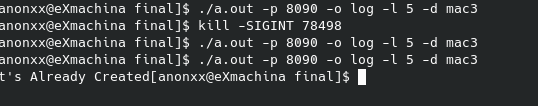
\includegraphics[width=\textwidth,height=\textheight,keepaspectratio]{images/doubleins.png} \\
Program runs in background as daemon process you can see ps -aux result\\
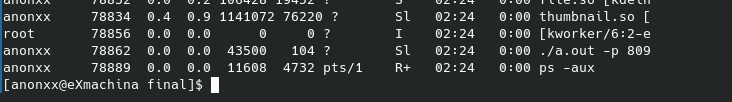
\includegraphics[width=\textwidth,height=\textheight,keepaspectratio]{images/deamon.png}\\As below you can see output for just one client\\
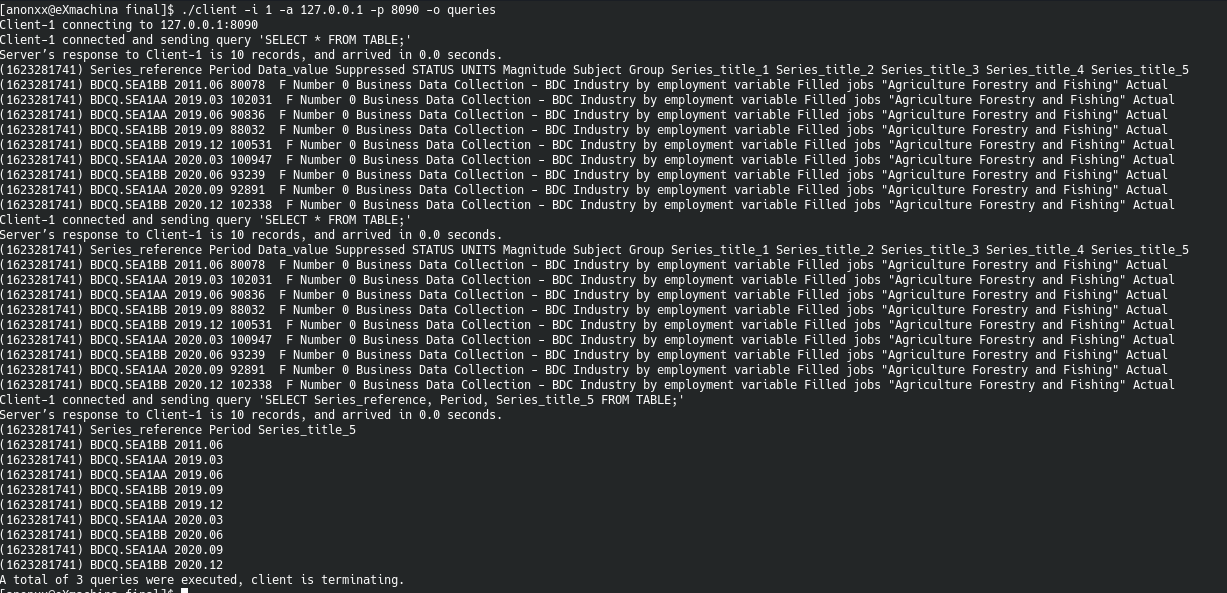
\includegraphics[width=\textwidth,height=\textheight,keepaspectratio]{images/clientout.png}\\Below you can see for the update operation\\
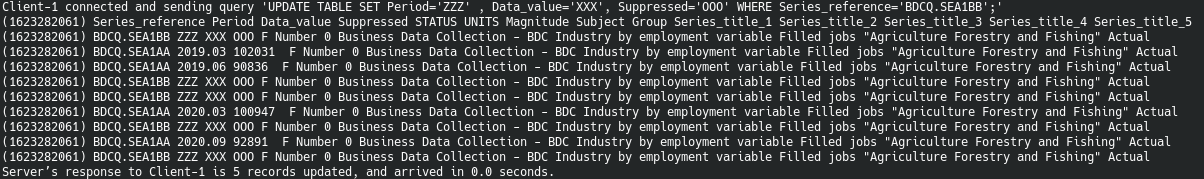
\includegraphics[width=\textwidth,height=\textheight,keepaspectratio]{images/cliupdated.png}\\There are some queries which is created by me \\
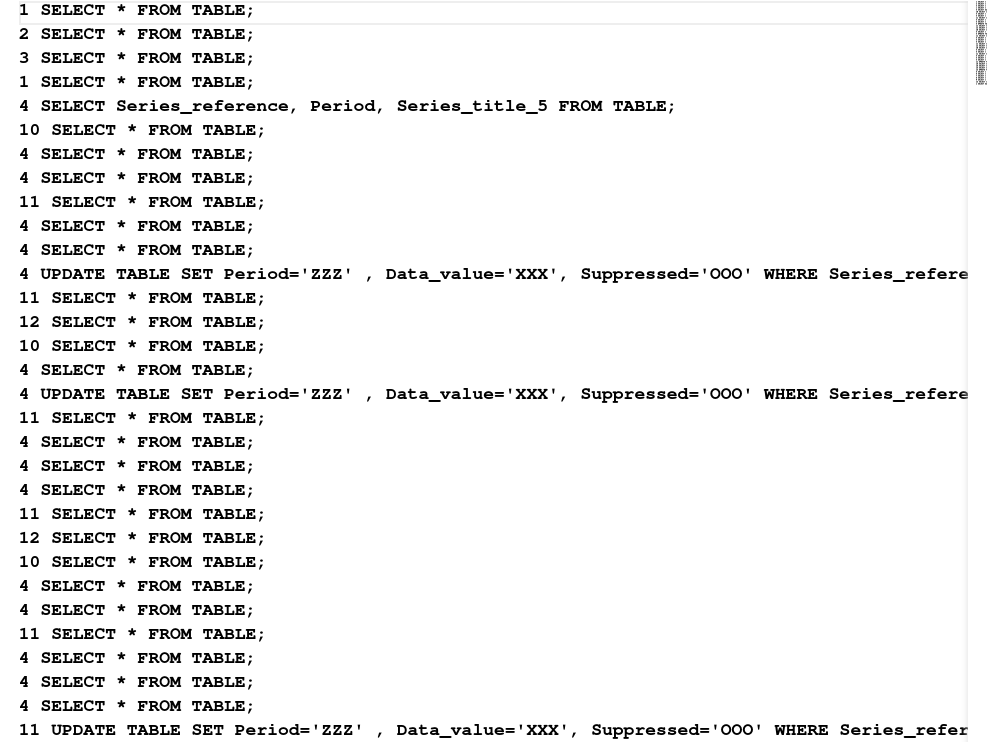
\includegraphics[width=\textwidth,height=\textheight,keepaspectratio]{images/queries.png}\\ there is a script file which includes 16 client also there is 5 or 6 threads\\
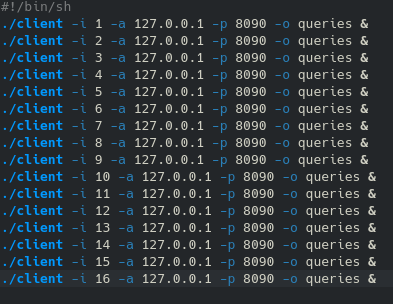
\includegraphics[width=\textwidth,height=\textheight,keepaspectratio]{images/script.png}\\ we can see by log file just 16 times we get delegated message which means for each client just one thread was busy\\
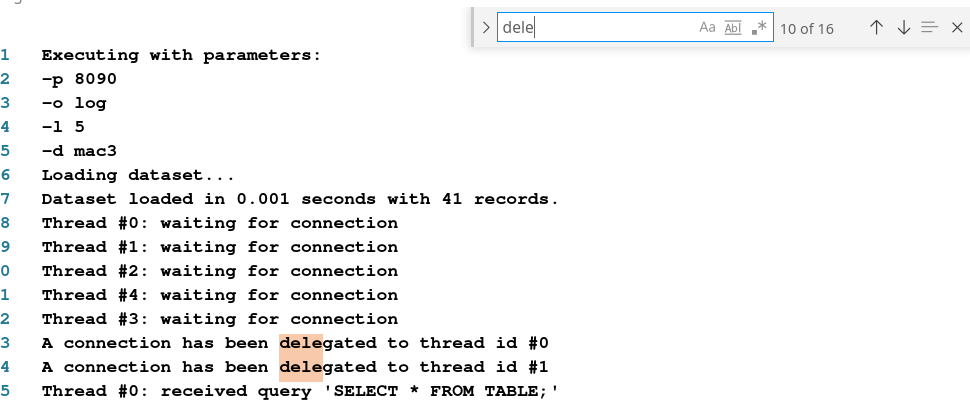
\includegraphics[width=\textwidth,height=\textheight,keepaspectratio]{images/delegated.png}\\ the number of query  which is 42 as in queries file\\
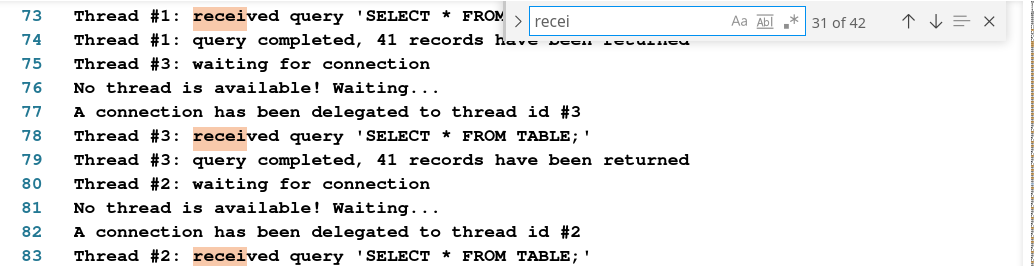
\includegraphics[width=\textwidth,height=\textheight,keepaspectratio]{images/received.png}\\ there is 42 result returned that means each queries has done\\
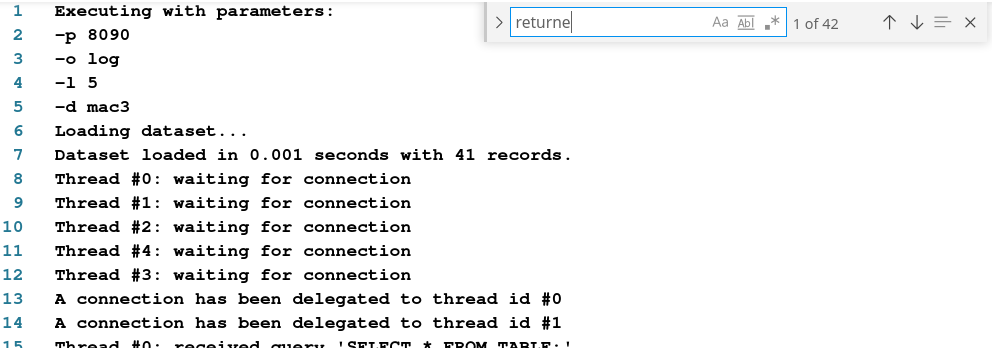
\includegraphics[width=\textwidth,height=\textheight,keepaspectratio]{images/returned.png}\\ when the Server gets SIGINT signal it prints that to the log file\\
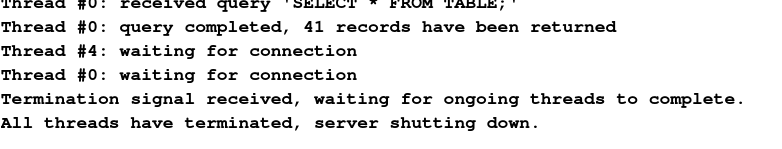
\includegraphics[width=\textwidth,height=\textheight,keepaspectratio]{images/shutdown.png}

{\huge \textbf{The Requirements I have achieved} \\}
{\large It provides all requirements but one }
 {\large I tried the rules below and they worked properly on my computer}
 
\begin{enumerate}
    \item {\large No compilation error }
    \item {\large No compilation warning}
    \item {\large \check{Makefile} }
    \item {\large \check{Report in Latex format}}
    \item {\large Printed usage information in case of missing or invalid argument}
    \item {\large Program did not crashed}
    \item {\large No zombie process}
    \item {\large No deadlock}
    \item {\large No poor synchronization}
    \item {\large Submitted on time}
    \item {\large Informed user in case of system errors}
    \item {\large ...}
    
\end{enumerate}

{\huge \textbf{The Requirements I have failed} \\}

{\large \\Since i could not manage the time i can not implement SELECT DISTINCT so don't try the query files which includes DISTINCT operations, Algorithm was ready bu I could not do that because of insufficient time( The idea was after get the value I will create a  column and mark them if it occurs second time so when i send it I would just send the unmarked rows of that column)}


\end{document}
